

\chapter{Physical Layer Neural Network Framework for Training Data Formation}
\label{chapter3}
\section{Abstract}
In this paper, we propose a low decay, low bias dataset synthesis framework that models Machine Learning (ML) dataset theory using Python classes and instruction files, and whose simulation results show an 11.58\% entropy decrease at classification time relative to state-of-the-art training sets. The demand for signal-domain Neural Networks (NNs) have increased significantly in recent years with respect to the classification of observed radio activity. In particular, there has been a growing interest in choosing appropriate training data in order to enhance NN performance at classification time. Developing ML based signal classifiers requires training data that captures the underlying probability distribution of real signals. To synthesize a set of training data that can capture the large variance in signal characteristics, a robust framework that can support arbitrary baseband signals and channel conditions is presented.


\section{Introduction}
\label{sec1}

\begin{figure*}[ht!]
	\centering	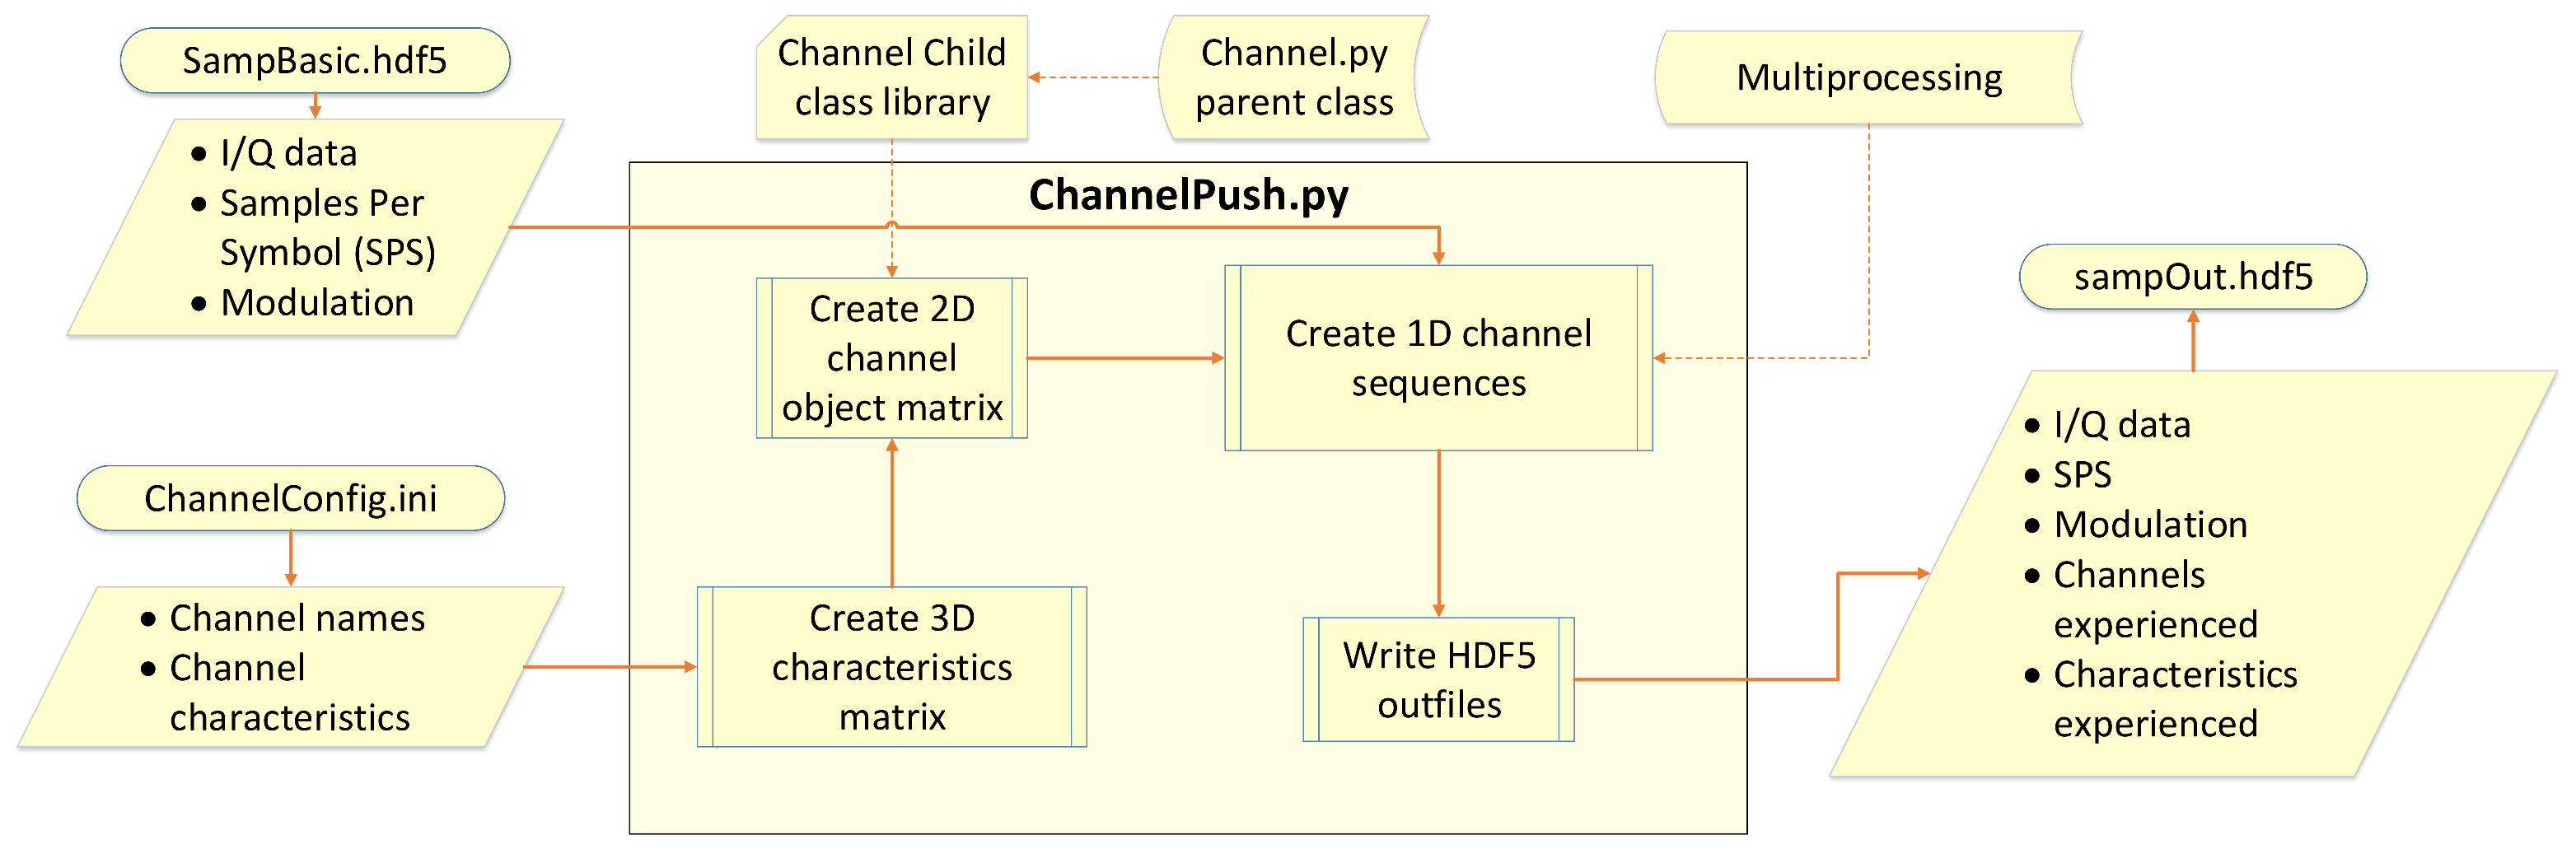
\includegraphics[width=1\textwidth,keepaspectratio]{figs/channelpush_poster.eps}
    \caption{Illustration of the proposed framework and the ChannelPush.py script. SampBasic.hdf5 acts as the Dataset Under Test (DUT) while ChannelConfig.ini as the instructions file. SampOut.hdf5 files are written as outputs. The 3D matrix is formed by the instructions file, containing the 2D matrix's (see Table \ref{table:tab3}) instance variables. The 2D matrix objects are formed by run-time channel class imports. 1D channel sequences (see Figure \ref{fig:1dlist}) are formed by permuting the channel imperfection objects from the 2D matrix, and the DUT is pushed sample by sample through each sequence in parallel.} 
\label{fig:channeltoolsub}      
\end{figure*}

Radio Frequency (RF) Neural Networks (NN) have recently received significant attention within the wireless research community~\cite{wang2017deep, 8054694}. However, RF NNs do not possess the openly available datasets and established benchmarks that are frequently associated with other NN applications~\cite{o2016radio, wang2017deep}. Consequently, there is a need within the wireless community for establishing freely available datasets and benchmarks that can be used to evaluate and compare the implementations of RF NNs.

In a dense RF environment, a receiver must be able to first detect and isolate a transmission~\cite{pahlavan2005wireless} before a RF NN
can extract features and perform signal classification. This detection and isolation is impeded by a variety of real-world impairments~\cite{tsb88tia, rappaport1996wireless}, which can negatively affect a NNs classification accuracy in highly time-varying and probabilistic environments. In recent publications \cite{o2016radio, 8170853}, the effect on evaluation-time classification accuracy of signal bandwidth (BW),
limits and statistics of powerful imperfections, and size of training sets has been explored but not fully understood.

For any signal-domain NN, an often used framework for dataset generation is the GNU Radio Companion (GRC) channel model blocks~\cite{o2016radio}. Each channel block offers a modular, sequential, and parallelized method of dataset manipulation. However, GRC cannot readily construct massive ensembles of varied wireless channels. Another resource for RF NNs is the RadioML 2016.10A dataset and Github repository, which contains their generation code~\cite{o2016radio}. While the dataset is popular due to its availability, some researchers have had difficulty in replicating the peak accuracy of their classifier~\cite{o2016convolutional}, and the statistics of the datasets are bound to a single, time-invariant channel model. Should a test set stray too far in terms of Signal-to-Noise-Ratio (SNR), pulse shaping, Local Oscillator (LO) drift, or some other parameter, the classification accuracy can potentially suffer~\cite{8170853} as a result of data bias, or training under a false assumption. A strength of signal-domain ML is that it is easy to simulate more data in order to grow a dataset. Consequently, as long as the memory and computational resources exist, generating large datasets that cover numerous permutations of channel imperfections would be a valuable tool with respect to the classification of real signals.

The work presented in this paper possesses the following contributions to the current state of the art:
\begin{itemize}
  \item A brief list of desirable variations for signal-domain ML datasets to achieve full coverage of the statistics of real signals.
  \item A framework that synthesizes datasets with the objective of reducing data decay and data bias, and capturing the underlying statistics of real signals.
\begin{itemize}
	\item Channel imperfection models are sequentially applied to input baseband signals modularly, where channel imperfections' constants and random variables (RV) are defined through the use of an instructions file.
\end{itemize}
  \item Example transmissions synthesized with our framework, constrained by parameters corresponding to relevant hardware specifications and signal structures.
  \item Simulation results showing that the generated datasets contain low entropy at evaluation time, and guidelines for generating diverse and robust RF-domain datasets through Kullback-Leibler Divergence (KLD) entropy analysis of approximations of Probability Density Functions (PDFs).
\end{itemize}

The rest of this paper is organized as follows: The proposed framework and dataset variations are presented in Section~\ref{sec2}, and applications of the framework in Section~\ref{sec3}. Section~\ref{sec4} presents KLD entropy analysis of training set approximations of PDFs and their implications on training set size, and concluding thoughts are presented in Section~\ref{sec5}.


\section{Proposed Framework}
\label{sec2}

The proposed framework is described in Figure~\ref{fig:channeltoolsub}. The framework requires a Dataset Under Test (DUT) as well as instructions for which channel imperfection models are to be applied to the DUT. The framework outputs are instances of the DUT that have been modified by a unique permutation of channel imperfections. Channel imperfection models may be added, modified, or removed from the framework by minimal editing of the instructions. Each 1D sequence's output is computed and written in a separate Central Processing Unit (CPU) process.

Regarding the size of an RF dataset and the choice of information it should contain, two pitfalls that need to be avoided when building a dataset for ML use are data decay and data bias, which are defined as follows:
\begin{itemize}
	\item \textit{Data decay} is the gradual decrease in testing accuracy over time as simulated training data and empirical testing data have statistically drifted apart. In the RF domain, data decay can be caused by hardware advances or changes in communication standards.
    \item \textit{Data bias} is any large difference in training and testing accuracy due to the training set being designed based on false assumptions. Examples for this are numerous, ranging from false assumptions about Signal-to-Noise-Ratio (SNR) and other channel characteristics to false assumptions about hardware condition and use.
\end{itemize}    
A framework is useful for the prevention of data decay since it allows for flexible and easy generation, keeping datasets current and relevant. Data bias can be avoided through the use of a framework by influencing training data by a wider range of effects than expected at evaluation time. A framework makes this tuning process simple and quick using small edits to an instructions file designed to maximize the amount of information contained in commands relevant to data bias and decay (\textit{i.e.}, link budget parameters).

\begin{table}[ht!]
\centering
\caption{Example 2D Channel Object Matrix (refer to Figure~\ref{fig:channeltoolsub}). Objects are instances of run-time imported Carrier Frequency Offset (CFO) and Additive White Gaussian Noise (AWGN) Python classes. Instance variables of the objects are imported from the 3D characteristics matrix. Some characteristic sweeps should be linearly spaced (phase ambiguity in radians), and others log spaced (SNR of an AWGN model)} 
\label{fig:channeltoolstructure}
\begin{tabular*}{1\textwidth}{c l c c}
\toprule
Channel & Feature & Variations & \\\hline
1&AWGN1 & Variance: 0.01 & SNR: 0 dB\\
&AWGN2 & Variance: 0.01 & SNR: 20 dB\\
&AWGN3 & Variance: 0.1 & SNR: 0 dB\\
&AWGN4 & Variance: 0.1 & SNR: 20 dB\\\hline
2&CFO1 & offset norm to samp rate: 2.5\% &\\
&CFO2 & offset norm to samp rate: 5.0\% &\\
\bottomrule
\end{tabular*}
\label{table:tab3}
\end{table}

ML datasets have $K$ categories (or labels), $y = \{0, 1,...,K-1\}$, and $N$ examples (\textit{i.e.}, images, text blocks, or an RF waveform) of dimensionality $D$, $x = \lbrack N \times D \rbrack$ \cite{cs231}. In the context of a modulation classifier of IQ datasets, $K$ is the number of modulation schemes to be used as labels, $D$ is the dimensions of a training signal, with a length equal to the number of complex samples per signal and a depth of 2 representing the in-phase and quadrature components of each complex sample, and $N$ is the number of transmissions in the dataset.

\begin{figure}[ht!]
	\centering	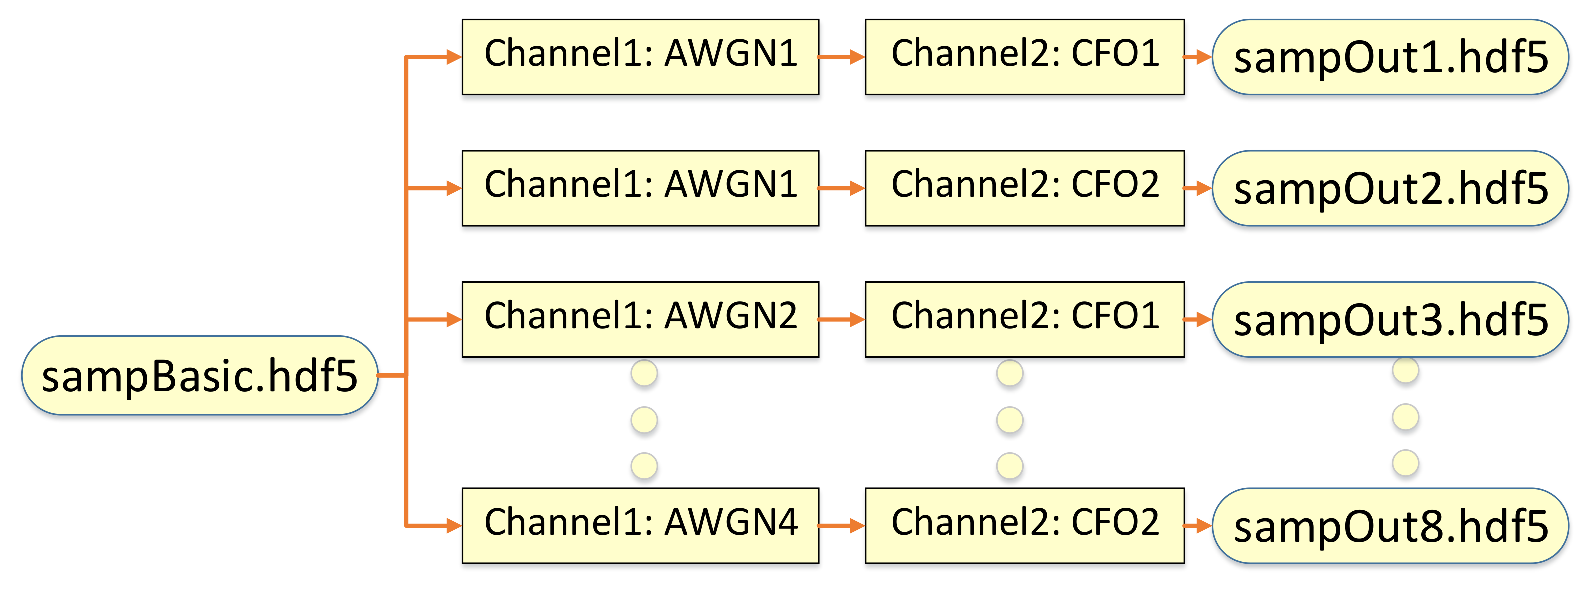
\includegraphics[width=1\textwidth,keepaspectratio]{figs/1d_list_poster.eps}
    \caption{Example set of eight 1D channel sequences (refer to Figure~\ref{fig:channeltoolsub}) formed by permuting through the 2D channel object matrix. SampBasic.hdf5 is the DUT, and is pushed through each sequence sample by sample, leveraging Multiprocessing.} 
\label{fig:1dlist}      
\end{figure}

Statistical heuristic methods of varying complexities suggest different amounts of data to fully represent the underlying statistics of a set of transmissions for the purpose of classification~\cite{75512}. A popular and simple heuristic that we consider represents the number of training examples $N$ as the product:
\vspace{-5mm}
\begin{subequations}
\begin{align}
N = K \times C
\\
C = (f \times F) \times (v \times V)
\end{align}
\end{subequations}


\noindent where $C$ is the number of training transmissions per class, $F$ is the number of transmissions per input feature the dataset has, $V$ is the number of transmissions per variation of those input features, and $f$ and $v$ are the number of input features and variations. The robust computer vision datasets CIFAR-10 and CIFAR-100~\cite{cifar} choose a $C$ value of 6,000 and 600, respectively, and the RF dataset RML2016.10A 1,000~\cite{8054694}.

To avoid data bias, one wants to include as many channel imperfections in training transmissions as possible in a signal-domain ML training set to avoid training under a false set of assumptions of channel conditions (see Table~\ref{tab:visionsignal} for examples). It is important to note that not all of these input features will have a significant effect on evaluation time accuracy, which is why the framework is designed to easily add and remove channel imperfection models, which rescales the number of training examples size by an integer change of:
\vspace{-1mm}
\begin{equation}
\Delta N = (\Delta f \times F) \times (\Delta v \times V).
\end{equation}

\noindent While several input variations are displayed in this paper, the proposed framework is designed with the explicit future purpose of allowing for an endless contribution of channel imperfection models from the physical layer ML community in addition to the list in Table~\ref{tab:visionsignal}.

Many features have well defined classical models that describe their behavior, excluding certain non-linear phenomenon such as amplifier non-linearities~\cite{wymeersch2007iterative}. It is the goal of this proposed framework to treat each one of these channel model imperfections as functions $f(a,b,...)$ described by variations $a,b,...$, which serve as function inputs.

\begin{table}[ht!]
\centering
\caption{Examples of variations in computer vision image datasets, and a collection of analogies for their signal domain parallel~\cite{cs231}.} 
\begin{tabular*}{1\textwidth}{c l c}
\toprule
Computer Vision & Communications \\\hline
Orientation & Phase ambiguity\\
Size & Signal amplitude\\
Deformation & AWGN, STO, more\\
Lighting & Frequency-fading multi-path\\
Occlusion & Signal jamming\\
Camouflaged & Co-band, neighbor-band interference\\
Intra-class Variation & Alternate modulation (i.e. non-rect QAM)\\
Image stretching & IQ imbalance\\
Motion Blur & Frequency offset (i.e. CFO, Doppler shift)\\
\bottomrule
\end{tabular*}
\label{tab:visionsignal}
\end{table}

In the proposed framework, the choice of features and variations to be used in an experiment are described by the instructions file. Instruction files have two lines of code per channel imperfection model, with one describing a key-value pair of the imperfection's name, and the other a key-value pair describing the imperfection model's function inputs (variations).


\section{Applications of Proposed Framework}
\label{sec3}

\begin{figure*}[ht!]
	\centering	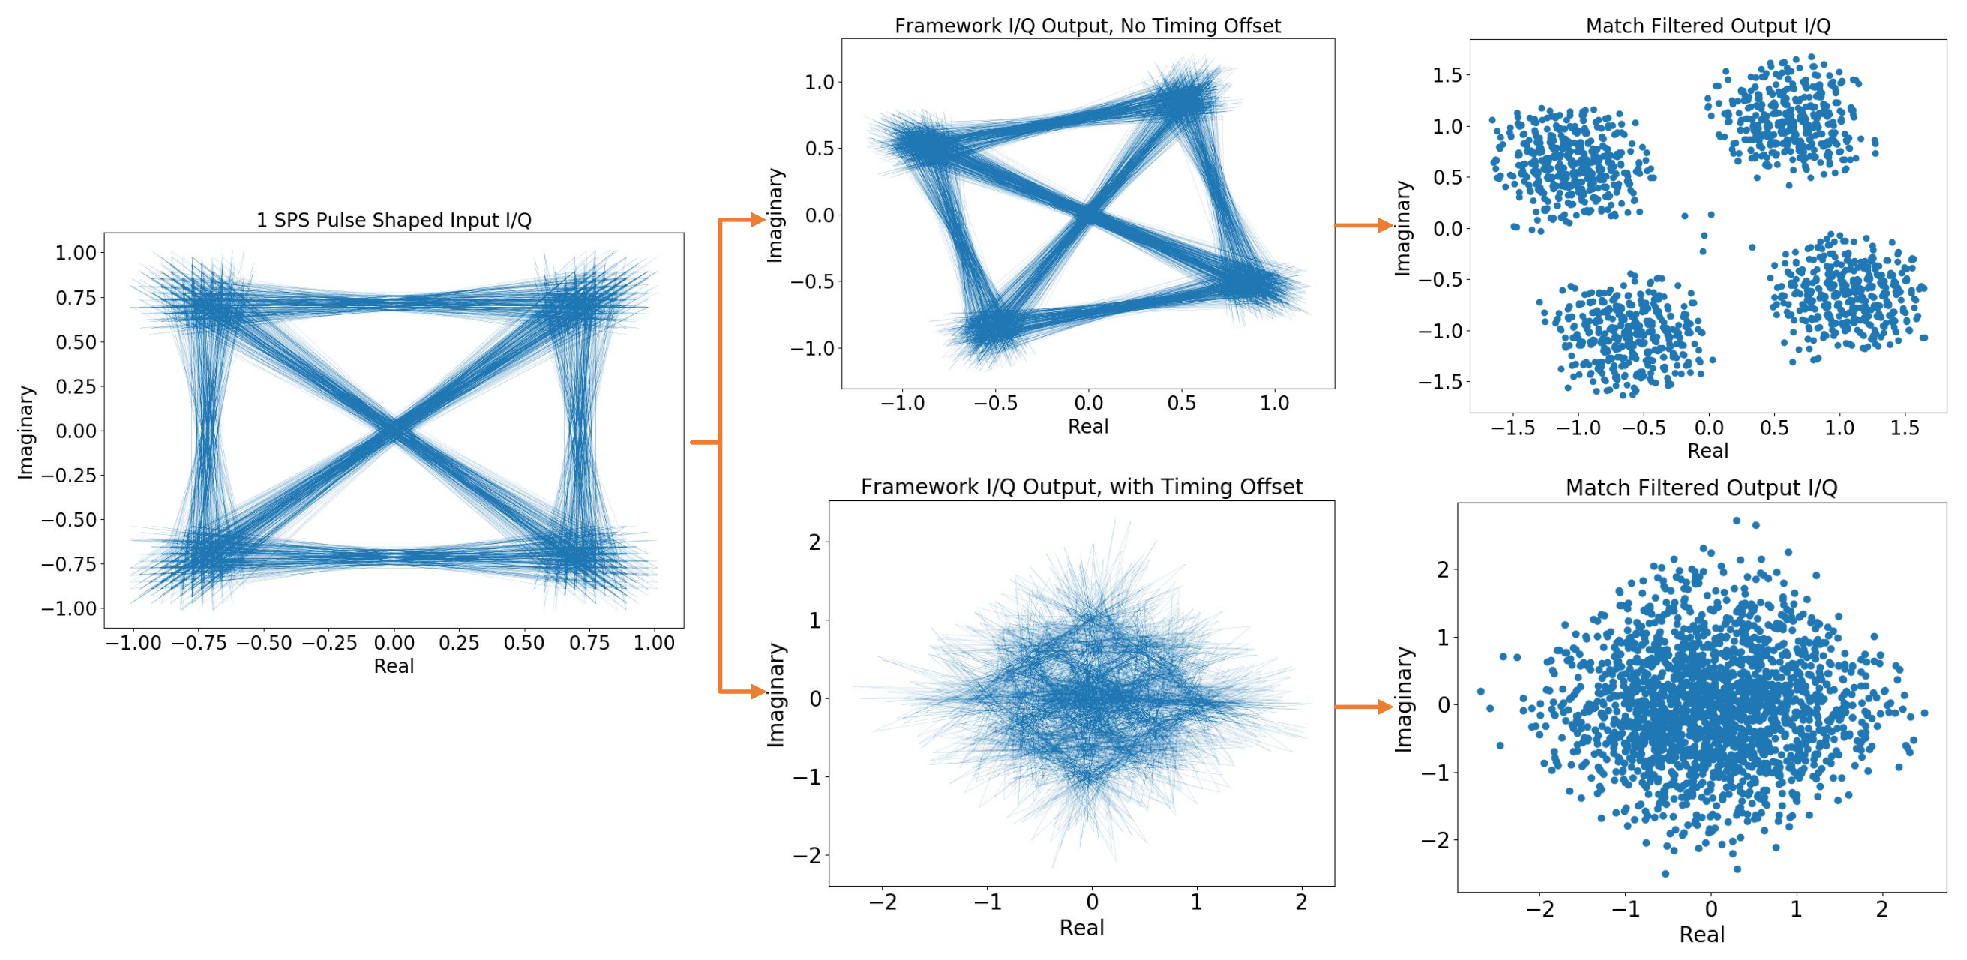
\includegraphics[width=1\textwidth,keepaspectratio]{figs/final_n210.eps}
    \caption{1 SPS pulse shaped Quadrature Phase-Shift Keying (QPSK) IQ data representing the baseband data of an Ettus Research N210 transmission. For the sake of visualization, frequency offset from Local Oscillator (LO) drift has been left out. The top track displays the dataset influenced by phase ambiguity and AWGN, then the matched filtering of that data. The bottom track additionally shows STO, where the data is interpolated and filtered up to an intermediate 2 SPS, offset in time, then decimated (and once again match filtered like the top track).} 
\label{fig:1spsslides}      
\end{figure*}

\begin{figure}[ht!]
\centering	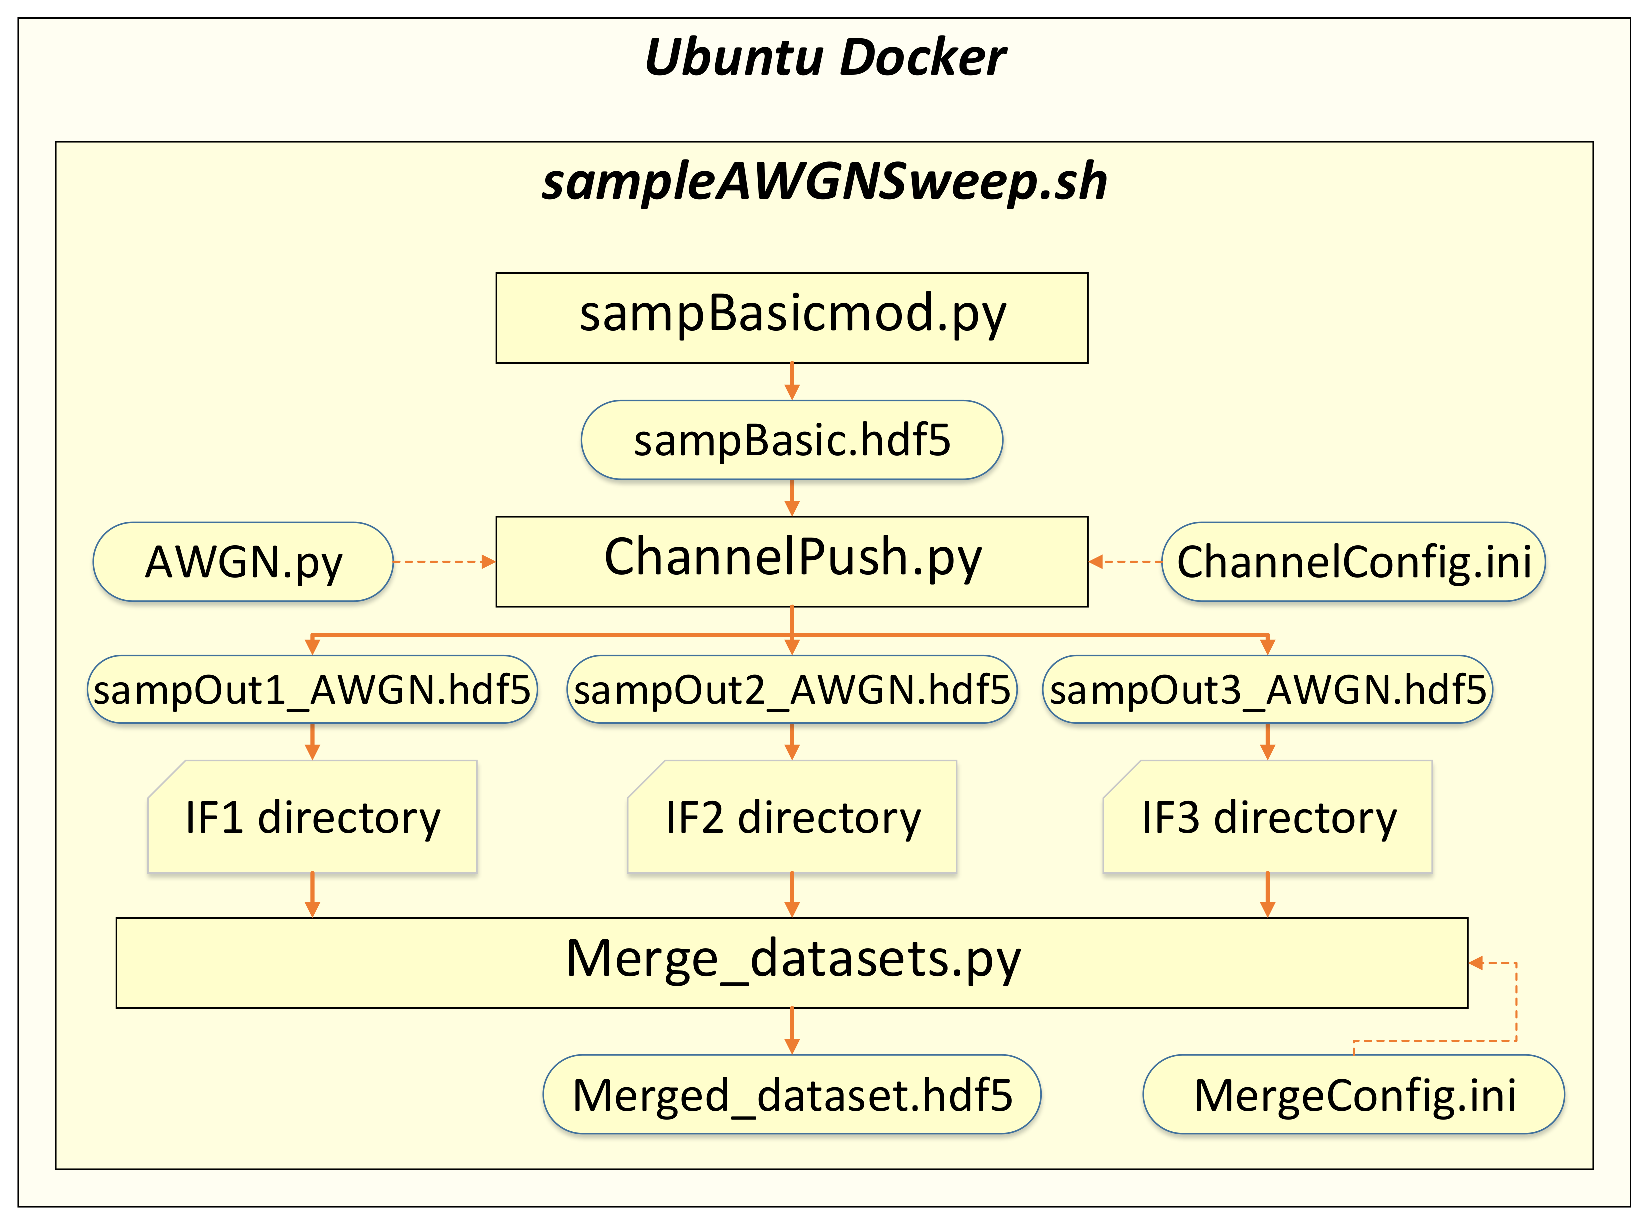
\includegraphics[width=1\textwidth,keepaspectratio]{figs/bashcmd_poster.eps}
    \caption{The AWGN channel effect is described by its SNR and Gaussian RV variance, $\sigma$. Three AWGN channels of varying SNR but constant $\sigma$ described by ChannelConfig.ini are applied to the same infile sampBasicmod.py. The outputs of which are manually moved to Intermediate Frequency (IF) folders corresponding to a secondary instructions file, MergeConfig.ini. Merge\_datasets.py (see Figure~\ref{fig:merge/}) modulates and sums the independent transmissions.} 
\label{fig:bashcmd_poster/}      
\end{figure}

\begin{figure}[ht!]
	\centering	\includegraphics[width=1\textwidth,keepaspectratio]{figs/merge_flow.eps}
    \caption{Three 16 SPS pulse shaped QPSK datasets from Figure~\ref{fig:bashcmd_poster/} are modulated to intermediate frequencies 10, 15, and 20 MHz. Each dataset was pushed through the framework as a DUT and modified by a unique AWGN channel block independently, each representing a transmitted signal. Future work will implement this feature to produce MIMO and OFDM datasets.} 
\label{fig:merge/}      
\end{figure}

In order to obtain real-world wireless data, we used in this work a USRP N210 software-defined radio (SDR) from Ettus Research employing an SBX daughter board~\cite{6815911}. Datasets influenced by state-of-the-art radio front-end imperfection models are valuable because the radios are current and widely-used, and thus the datasets are resistant to data decay and bias. In this instruction file, imperfection models are defined by data sheets describing the Ettus N210 with an SBX daughter-board~\cite{n210sbx}. Figure \ref{fig:1spsslides} illustrates an example transmission from the dataset, $x_i$ of dimensionality $D$, where each sample of $x_i$ is a complex tuple (I, Q). Each $x_i$ represents a transmission sent from an N210 impacted by CFO, AWGN, STO, and phase ambiguity, the four of which are believed by the authors to be amongst the most influential RF variations on IQ shape and behavior, and thus evaluation-time accuracy of real signals.

Most RF environments are not occupied by a single signal, but by a dense clutter of unique signals organized by time-varying Medium Access Control (MAC) and network-layer protocols. Consequently, certain channel imperfections such as multi-path fading can be correlated across multiple transmissions (\textit{i.e.}, due to common landmarks), while imperfections such as a transmitter and receivers LO drift are statistically independent. To synthesize training and testing sets that use state-of-the-art signal structures, these imperfections need to be appropriately correlated and applied, and their transmissions summed. Figure \ref{fig:bashcmd_poster/} presents a set of three separate transmissions produced from the proposed framework in pursuit of this goal.


\section{Simulations and Results}
\label{sec4}

In the previous section, we discussed the number of examples a training set should have and what information those examples should contain. As shown in~\cite{8170853}, the number of observations or samples that are contained in an example can have a significant impact on training time and testing accuracy of a NN. In this section, we will investigate how many samples pulled from RVs are needed to estimate their theoretical PDFs to within a specific degree of accuracy.

It is desirable to have the number of samples be integers of base two since it is computationally efficient~\cite{cs231} and allows for an integer number of symbols to be contained in each training example, as most commonly SPS is also base two. Furthermore, each training example needs to create enough instances of the RVs that govern its variations such that a PDF formed from that data is similar to the theoretical PDF. In this way, testing data can be correctly classified because the NN has learned the behavior of the data. The Central-Limit Theorem (CLT) states that when properly normalized, independent RVs are summed, the distribution tends towards a Gaussian one. Furthermore, the Law of Large Numbers states that the average result of a certain number of trials tends towards the expected value as the number of trials increases. To investigate the implications of these two laws in signal-domain dataset synthesis as they pertain to Figure~\ref{fig:1spsslides}, we perform the KLD analysis (\ref{eq:KLD}) in Figure~\ref{fig:kldiv}:

\begin{equation}
\label{eq:KLD}
D_{KL}(P||Q) = \sum_{i} P(i) log_2\bigg(\frac{P(i)}{Q(i)}\bigg),
\end{equation}

\noindent where the expected probability $P(i)$ can be defined as the definition of a Gaussian PDF:

\begin{equation}
\label{eq:pi}
P(i) = \frac{1}{\sqrt{2\pi\sigma^2}} e^{-\frac{(x-\mu)^2}{2\pi\sigma^2}},
\end{equation}

\noindent and the measured probability $Q(i)$ is defined as the histogram formed from the data $q(i)$:

\begin{equation}
\label{eq:qi}
q(i) = CDF_{norm}^{-1}(u) + eps,
\end{equation}

\noindent where $eps \thicksim U(0,0^+)$ to avoid $log_2(0)$ errors in (\ref{eq:KLD}) resulting from zero-observation bins, $u \thicksim U(0,1)$, and $CDF_{norm}^{-1}(u)$ is the inverse Cumulative Distribution Function (CDF) of the Gaussian distribution:


\begin{equation}
\label{eq:cdfinv}
CDF_{norm}(x) = \frac{1}{2} \bigg[ 1 + \erf \frac{x - \mu}{\sigma\sqrt{2}}\bigg].
\end{equation}

\begin{figure}[ht!]
	\centering	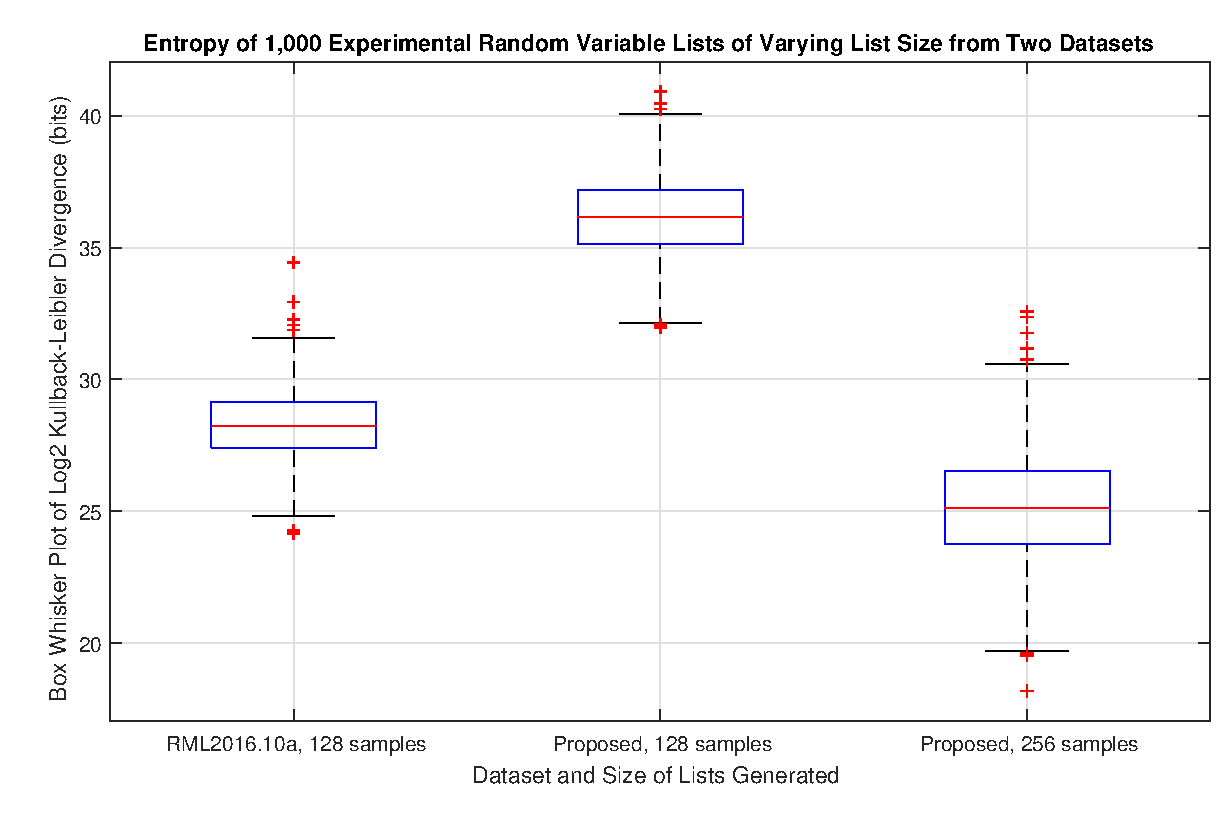
\includegraphics[width=1\textwidth,keepaspectratio]{figs/kldiv.eps}
    \caption{RML2016.10A is composed of 1,000 training sets containing 128 samples each per class per SNR value. Transmissions average 28.3 bits divergence from theory. The proposed application (see Figure~\ref{fig:1spsslides}) averages 36.2 bit divergence from theory. In order to achieve similar KLD entropy at an RF NNs evaluation time to state-of-the-art datasets, this analysis shows our proposed application requires at least 256 samples per transmission. The resulting divergence from theory is 25 bits, or a 11.58\% decrease from RML2016.10A.} 
\label{fig:kldiv}      
\end{figure}


\noindent RML2016.10A is a dataset generated using GRC's dynamic channel model, which combines their Symbol Rate Offset (SRO), CFO, and flat-frequency fading models. The probabilistic nature of the dataset is dictated by the SRO and CFO Gaussian RVs, and the AWGN Gaussian RV. Our proposed application (see Figure~\ref{fig:1spsslides}) is described by a uniform RV from a phase ambiguity and STO model, two Gaussian RVs describing the CFO of a transmitting and receiving LO, and a Gaussian RV contained in the AWGN model. Since KLD is additive (\ref{eq:KLDadd}) for independent distributions (\textit{i.e.}, $P_1,P_2,Q_1,Q_2$), the values in Figure~\ref{fig:kldiv} are calculated as the sum of KLD for each RV of the dataset under consideration.

\begin{equation}
\label{eq:KLDadd}
D_{KL}(P||Q) = D_{KL}(P_1||Q_1) + D_{KL}(P_2||Q_2).
\end{equation}

\section{Conclusion}
\label{sec5}
Our proposed framework showcases the ability to model fundamental ML theory through the use of an instruction file and a library of Python classes. The proposed framework has low data decay and data bias, and the KLD entropy analysis shows that an application of our proposed framework achieves 11.58\% less entropy than state-of-the-art datasets at classification time.

